\newcommand{\SGBag}{\emph{(SGBag complet)}}
\newcommand{\SGBagP}{\emph{(SGBag partiel)}}
\newcommand{\Simu}{\emph{(Simulation)}}
\newcommand{\Proto}{\emph{(Prototype)}}
\let\phase\subsection

\section{Liste des livrables}
\phase{Étude préliminaire}
\begin{itemize}
	\item Liste organisée des besoins \SGBagP
	\item Modèle de domaine \SGBagP
\end{itemize}

\phase{Élaboration}
\begin{itemize}
	\item Modèle de cas d'utilisations \SGBagP
	\begin{itemize}
		\item Définition des acteurs
		\item Description textuelle
		\item Diagrammes
	\end{itemize}
	\item Modèle de cas d'utilisations \Simu
	\item Liste des scénarios \Simu
	\item Diagramme des paquetages d'analyse \SGBag
	\item Scénarios à réaliser dans la liste précédente \Proto
	\item Diagrammes de séquences en boîte noire (système vu de l'extérieur) des scénarios suivants \Simu{} :
	\begin{itemize}
		\item Arrivée manuelle d'un bagage
		\item Top d'horloge
	\end{itemize}
	\item Diagrammes de séquences en boîte grise (noyau détaillé) des scénarios suivants \Simu{} :
	\begin{itemize}
		\item Arrivée manuelle d'un bagage
		\item Top d'horloge
	\end{itemize}
	\item Modèle structurel (diagramme de classes) \Proto
\end{itemize}

\phase{Construction}
\begin{itemize}
	\item Diagrammes de séquence (boîte grise) de scénarios additionnels \Proto{} :
	\begin{itemize}
		\item Création d'un vol
		\item Association d'un vol
		\item Démarrer la simulation
		\item Passer en mode automatique
	\end{itemize}
	\item Diagramme de classe des vues
	\item Diagrammes de séquences (boîte blanche) suivants \Proto{} :
	\begin{itemize}
		\item Partie générique pour toute commande sur un élément
		\item Arrivée manuelle de bagage
		\item Changement de vitesse d'un tapis roulant
	\end{itemize}
	\item Modèle structurel complet (noyau et vues) \Proto
	\item Code source \Proto
	\item Exécutable \Proto
\end{itemize}

\phase{Transition}
\begin{itemize}
	\item Livrables organisationnels
	\item Commentaires
\end{itemize}


\section{Planning prévisionnel}
\newpage
\begin{figure}[H]
	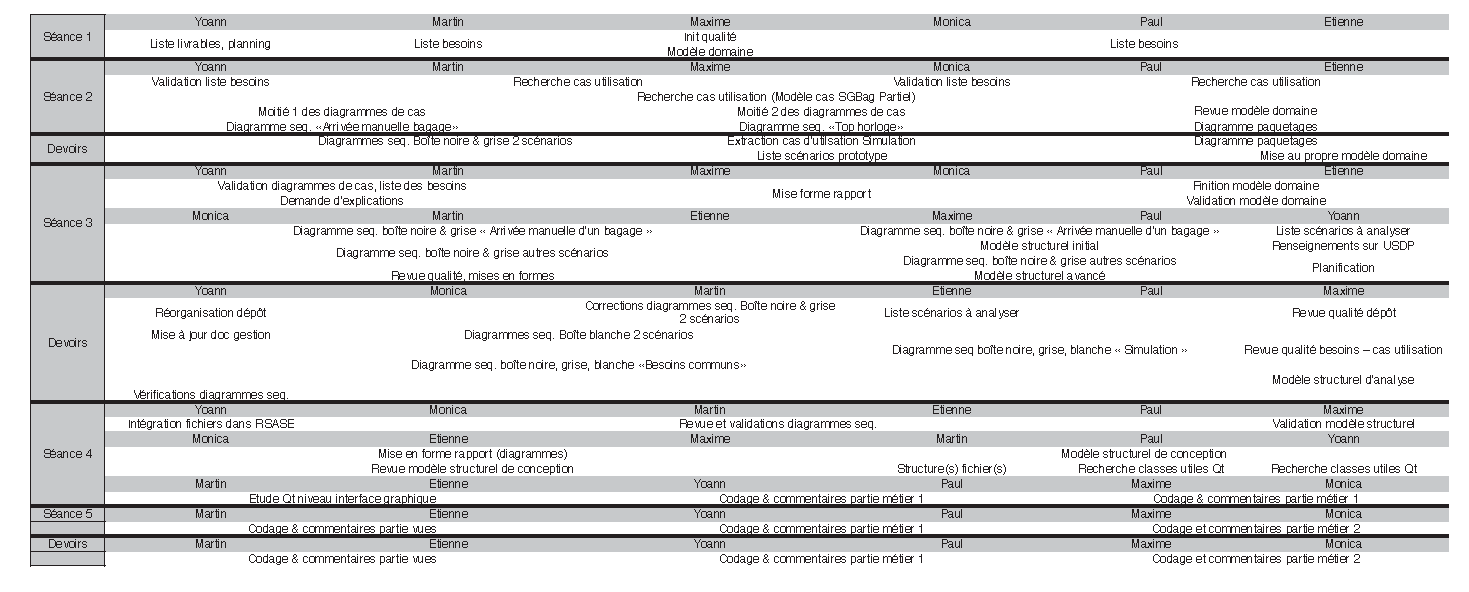
\includegraphics[width=\textwidth,angle=90]{planning1.pdf}
\end{figure}

